In diesem Abschnitt wird die Kaskadierungsvariante des Direct Cascade Netzwerks vorgestellt. Das Netzwerk ist hierbei vollständig vorab 
definiert und besteht aus einem einzelnen Hidden Layer sowie einem Output Layer. Die Gesamtstruktur setzt sich aus mehreren identischen 
Subnetzwerken zusammen, zwischen denen während des Trainings ein Wissenstransfer stattfindet.

\begin{figure}[htpb]
    \centering
    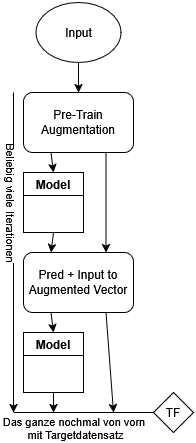
\includegraphics[height=10cm]{../../Graphiken/direct_cascade.png}
    \caption{\label{fig:directcascade} 
    \small{Hier wird das Direct Cascade Verfahren dargestellt. Dieses Verfahren verwendet mehrere einzelne Netzwerke 
    (hier als Modelle bezeichnet), die jeweils nur wenige Hidden Layer aufweisen, in der Regel lediglich einen. Nach der 
    Initialisierung und dem Training wird jedes Modell einmal ohne weiteres Training angewendet, dessen Ausgangssignal mit dem ursprünglichen 
    Eingabesignal kombiniert wird. Diese Kombination bildet den neuen Eingabedatensatz für das nachfolgende Modell. Durch diese sukzessive 
    Verknüpfung der Ausgaben mit den Eingaben kann das Verfahren eine Wissensweitergabe und -integration zwischen den einzelnen Modellen 
    realisieren. Darüber kann an beliebiger Stelle TF verwendet werden.}}
\end{figure}

Der Ablauf beginnt, wie in Abbildung \ref{fig:directcascade} dargestellt, mit dem vorbereiteten Source-Datensatz, der als 
Eingabe in die erste Instanz des Netzwerks gegeben wird. Diese Netzwerkinstanz wird anschließend trainiert. Nach Abschluss des Trainings 
erfolgt eine einmalige Anwendung des fixierten Netzwerks, deren Ergebnis die Vorhersage (Prediction) darstellt. Diese Prediction wird mit 
dem ursprünglichen Eingabesignal desselben Netzwerks kombiniert, wodurch ein sogenannter Augmented Vector entsteht. Die genaue Bildung dieses 
Augmented Vectors variiert dabei leicht je nach spezifischer Implementierung des jeweiligen Direct Cascade Netzwerks und wird an späterer 
Stelle detaillierter erläutert.

Der Augmented Vector dient als Input für die nächste Instanz des Netzwerks. Dieser Zyklus aus Netzwerkinstanz, Training, Prediction und 
Augmented Vector Berechnung wird beliebig oft wiederholt. Durch die Einbindung der Prediction in den Augmented Vector kann das Netzwerk 
Wissen aus den zuvor trainierten Instanzen übernehmen und integrieren.

TF kann jederzeit innerhalb eines Trainingsschritts durchgeführt werden, indem anstelle des Source-Datensatzes 
ein Target-Datensatz als Input verwendet wird. Dabei können beliebig viele Netzwerkinstanzen vor und nach 
TF genutzt werden. Der einzige Unterschied besteht darin, dass der Augmented Vector mit jedem weiteren Netzwerk etwas 
größer wird, da er sowohl das Wissen aller bisher trainierten Netzwerke als auch die ursprünglichen Eingabedaten enthält.

Für die Implementierung bedeutet dies, dass von Beginn an sowohl der Source- als auch der Target-Datensatz in das feste Netzwerk eingespeist 
werden müssen. Dies ist notwendig, um die Prediction auf dem Target-Datensatz – die während der Trainingsphase mit dem Source-Datensatz generiert 
wurde – im Augmented Vector zu integrieren. Somit wird sichergestellt, dass das während des Trainings auf dem Source-Datensatz gelernten 
Wissens auch bei der Anpassung an den Target-Datensatz berücksichtigt werden.
